\subsection{Generation of the reference panel by genotype refinement and phasing}
\label{sec:refine_and_phase}
We carry out genotype refinement and phasing with SHAPEIT2\cite{Delaneau2012} and MVNcall.\cite{Menelaou2013} We use the SHAPEIT2 for phasing of biallelic sites and MVNcall for phasing of multiallelic sites. We use SHAPEIT2, because it improves on the accuracy of phasing.\cite{2014Delaneau} Initial refinement of genotype likelihoods is carried out with Beagle4.\cite{Browning20071084} The posterior probabilities calculated by Beagle4 are then used as input for SHAPEIT2 and MVNcall along with a haplotype scaffold generated from SNP array data available for the same populations (figure \ref{fig:haplotype_scaffold}). The SNP array data undergoes QC per population and is phased with SHAPEIT2 across all populations to generate the haplotype scaffold.

\begin{figure}[!htbp]
\centering
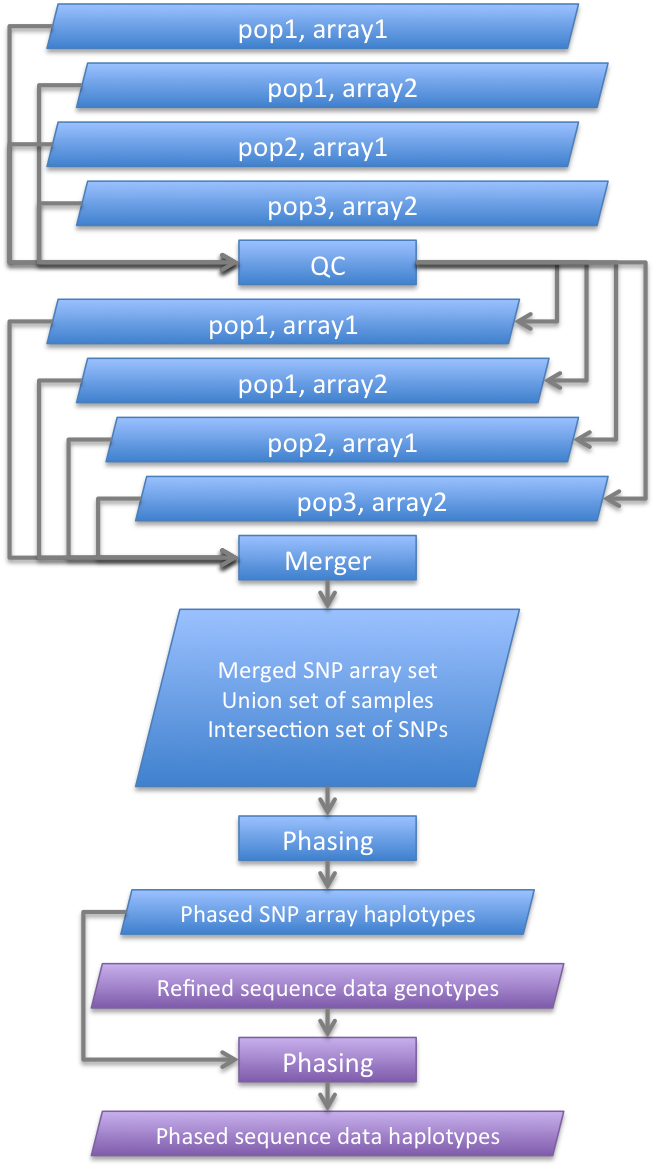
\includegraphics[width=0.4\textwidth]{haplotype_scaffold}
\caption{A haplotype scaffold is used for phasing of the sequence data. The haplotype scaffold is generated from highly accurate SNP array data available for sequenced samples and additional relevant samples and populations (summarized in table \ref{tab:samples_chip} on page \pageref{tab:samples_chip}).}
\label{fig:haplotype_scaffold}
\end{figure}

%MVNcall can also utilize a haplotype scaffold and unlike SHAPEIT2 works for multiallelic sites.\cite{Menelaou2013} However, we use SHAPEIT2, because it improves on the accuracy of phasing.\cite{2014Delaneau}
The Illumina Omni2.5M SNP array has been shown to be an optimal/sufficient haplotype scaffold size in African populations.\cite{Menelaou2013}\cite{2014Delaneau} Pedigree information will be used by SHAPEIT2 when available. For Beagle4 this is less important, as this is only an initial refinement used as input for SHAPEIT2 and MVNcall. We use the duoHMM method of SHAPEIT2 for phasing, because it has been shown to have a lower switch error rate, when pedigree information is available.\cite{OConnell2014} Following generation of this haplotype scaffold, SHAPEIT2 phases the sequence data by filling in missing data in between the scaffold, resulting in more accurate phasing of sequence data.

The chip data will undergo calling and quality control as previously\cite{Gurdasani2015} and as described in section \ref{sec:QCchip}. For the haplotype scaffold, in addition to in-house genotype data available, we will also use called chip data from the 1000G populations YRI (Yoruba in Ibadan, Nigeria) and LWK (Luhya in Webuye, Kenya), which are the only African populations alongside MKK (Maasai in Kinyawa, Kenya), which were genotyped on the Illumina Omni2.5M chip as part of 1000G.
%ftp://ftp.1000genomes.ebi.ac.uk/vol1/ftp/release/20130502/supporting/hd_genotype_chip/

We use the latest release (1274) of Beagle4. We use a sliding window size of 50000 variants and an overlap of 3000 variants between sliding windows. We use the default parameters; e.g. singlescale=0.8, duoscale=1.0, trioscale=1.0, burnin-its=5, phase-its=5, impute-its=5. We sample 4 haplotypes for each individual during each iteration of the algorithm (nsamples=4) and use 1200 variants to build the haplotype frequency model at each locus (buildwindow=1200). After refinement we check that there is a high concordance and correlation between SNP array genotypes and the refined sequence genotype posterior probabilities.

%Figure 8: Overall percent genotype discordance for different scaffold SNP density. Results are presented by population groups: African, European and Asian.
%Is MVNCall only better, if BEAGLE doesn't have phasing information?
%2014Delaneau - "It has been observed that the Beagle method does not have this property, and that Thunder and Impute2 benefit from using an initial set of haplotypes estimated via Beagle."
%2014Delaneu - "This approach generalizes our MVNcall, approach which is designed to phase one variant site at a time onto a haplotype scaffold, and improves upon its accuracy, by phasing multiple sites jointly onto the scaffold and using a more sophisticated underlying model."

%% https://mathgen.stats.ox.ac.uk/genetics_software/shapeit/shapeit.html#gcall